%%%%%%%%%%%%%%%%%%%%%%%%%%%%%%%%%%%%%%%%%%%%%%%%%%%%%%%%%%%%%%%%%%%%%%%%%%%%%%%%
%% MediHelp — A RAG-Powered Personal Health Assistant on a Microservice Backbone
%% B.Tech Major Project Thesis (IIEST Shibpur), 2026
%%%%%%%%%%%%%%%%%%%%%%%%%%%%%%%%%%%%%%%%%%%%%%%%%%%%%%%%%%%%%%%%%%%%%%%%%%%%%%%%

\documentclass[12pt]{caltech_thesis}

\usepackage[utf8]{inputenc}
\usepackage[T1]{fontenc}
\usepackage{newtxtext,newtxmath}
\usepackage{graphicx}
\usepackage{float}
\usepackage{caption}
\usepackage{subcaption}
\usepackage[hyphens]{url}
\usepackage{xcolor}
\usepackage{booktabs}
\usepackage{amsmath,amssymb,amsfonts}
\usepackage{algorithm,algpseudocode}
\usepackage{cite}
\usepackage{natbib}
\usepackage{ragged2e}
\usepackage{listings}
\usepackage[hidelinks]{hyperref}
\usepackage{tikz}
\usetikzlibrary{shapes.geometric, arrows.meta, positioning, fit, calc, backgrounds}

% Colour palette for architecture diagrams (matches the mermaid source in docs/architecture.md)
\definecolor{javafill}{HTML}{E3F2FD}
\definecolor{javastr}{HTML}{1976D2}
\definecolor{pyfill}{HTML}{E8F5E9}
\definecolor{pystr}{HTML}{43A047}
\definecolor{infrafill}{HTML}{F3E5F5}
\definecolor{infrastr}{HTML}{7B1FA2}
\definecolor{extfill}{HTML}{FFF3E0}
\definecolor{extstr}{HTML}{FF9800}

% TikZ styles
\tikzset{
  jbox/.style  ={rectangle, rounded corners, draw=javastr,  fill=javafill,
                 thick, minimum height=0.85cm, minimum width=1.7cm, align=center,
                 font=\footnotesize},
  pybox/.style ={rectangle, rounded corners, draw=pystr,    fill=pyfill,
                 thick, minimum height=0.85cm, minimum width=1.7cm, align=center,
                 font=\footnotesize},
  infrabox/.style={cylinder, shape border rotate=90, aspect=0.2,
                 draw=infrastr, fill=infrafill, thick,
                 minimum height=0.95cm, minimum width=1.5cm, align=center,
                 font=\scriptsize},
  qbox/.style  ={trapezium, trapezium left angle=70, trapezium right angle=110,
                 draw=infrastr, fill=infrafill, thick, minimum height=0.7cm,
                 align=center, font=\scriptsize},
  extbox/.style={rectangle, rounded corners, draw=extstr, fill=extfill,
                 thick, minimum height=0.7cm, minimum width=1.8cm, align=center,
                 font=\footnotesize},
  flow/.style  ={-{Stealth[length=2mm]}, thick},
  evt/.style   ={-{Stealth[length=2mm]}, thick, dashed, draw=infrastr},
}

% Code listing style
\lstset{
  basicstyle=\ttfamily\small,
  breaklines=true,
  frame=single,
  framerule=0.5pt,
  rulecolor=\color{gray!50},
  backgroundcolor=\color{gray!5},
  tabsize=2,
  showstringspaces=false,
  columns=fullflexible,
}

%%%%%%%%%%%%%%%%%%%%%%%%%%%%%%%%%%%%%%%%%%%%%%%%%%%%%%%%%%%%%%%%%%%%%%%%%%%%%%%%
%% CONFIGURE
%%%%%%%%%%%%%%%%%%%%%%%%%%%%%%%%%%%%%%%%%%%%%%%%%%%%%%%%%%%%%%%%%%%%%%%%%%%%%%%%

\newcommand{\thesistitle}{MediHelp: A RAG-Powered Personal Health Assistant on a Microservice Architecture}
\newcommand{\supervisorname}{Dr.~Tamal Pal}
\newcommand{\supervisorrank}{Assistant Professor}
\newcommand{\supervisordept}{Department of Computer Science and Technology}
\newcommand{\supervisorinstitution}{Indian Institute of Engineering Science and Technology, Shibpur}
\newcommand{\hodname}{Dr.~Apurba Sarkar}
\newcommand{\hodrank}{Associate Professor}
\newcommand{\degreename}{Bachelor of Technology in Computer Science and Technology}
\newcommand{\submissionyear}{2026}

\newcommand{\studentlist}{%
    Anushka Ghosh (2022CSB007),
    Shivam Rai  (2022CSB011),
    Ritabrata Bhattacharya (2022CSB024),
    Debosmita Pal (2022CSB029),
    Souvik Jha (2022CSB030),
    Subhrajit Deb (2022CSB032),
    and Aditi Karmakar (2022CSB046)%
}

\begin{document}

\title{\thesistitle}
\author{\studentlist}
\degreeaward{\degreename}
\university{\supervisorinstitution}
\address{Howrah, West Bengal}

%%%%%%%%%%%%%%%%%%%%%%%%%%%%%%%%%%%%%%%%%%%%%%%%%%%%%%%%%%%%%%%%%%%%%%%%%%%%%%%%
%% CERTIFICATE
%%%%%%%%%%%%%%%%%%%%%%%%%%%%%%%%%%%%%%%%%%%%%%%%%%%%%%%%%%%%%%%%%%%%%%%%%%%%%%%%

\begin{center}
\textbf{\LARGE Certificate}
\vspace{2cm}
\begin{flushleft}
This is to certify that \textbf{\studentlist} have successfully completed the
Major Project titled \textbf{\thesistitle} under my supervision.

\vspace{0.5cm}
The project was carried out as a partial fulfillment of the requirements for
the award of the degree of \textbf{\degreename}, \submissionyear.
\vspace{2cm}
\end{flushleft}

\noindent\begin{flushleft}Date: \rule{5cm}{0.4pt}\end{flushleft}
\vspace{2cm}

\begin{flushright}
    \rule{7cm}{0.4pt}\\
    Signature of Supervisor\\
    \supervisorname\\
    \supervisorrank,\\
    \supervisordept,\\
    \supervisorinstitution
\end{flushright}
\end{center}

%%%%%%%%%%%%%%%%%%%%%%%%%%%%%%%%%%%%%%%%%%%%%%%%%%%%%%%%%%%%%%%%%%%%%%%%%%%%%%%%
%% ACKNOWLEDGEMENTS + ABSTRACT
%%%%%%%%%%%%%%%%%%%%%%%%%%%%%%%%%%%%%%%%%%%%%%%%%%%%%%%%%%%%%%%%%%%%%%%%%%%%%%%%

\begin{acknowledgements}
   We extend our sincere gratitude to our supervisor \textbf{\supervisorname},
   \supervisordept, for the invaluable supervision, technical guidance, and
   unwavering support extended throughout this project. The freedom we were
   given to explore architectural choices --- from cloud-hosted to fully
   self-hosted deployments, from monolithic to microservice decompositions ---
   shaped both the project and our understanding of real systems engineering.

   We also thank \textbf{\hodname}, \hodrank{} and Head of \supervisordept,
   and the faculty and staff of \supervisorinstitution{} for fostering an
   environment in which
   ambitious, end-to-end student projects are encouraged. Special thanks to
   our peers who participated in informal user testing and whose feedback
   surfaced bugs we would have otherwise missed before submission.

   Finally, we acknowledge the open-source ecosystems that made this project
   feasible at zero capital cost: Spring Boot, Spring Cloud Netflix, Angular,
   Flask, LangChain, HAPI~FHIR, Pinecone, Groq, and the Apache Software
   Foundation.
\end{acknowledgements}

\begin{abstract}
We present \textbf{MediHelp}, a personal health-assistant web application
that addresses the full care cycle --- pre-diagnosis support, post-appointment
monitoring, prescription management, and continuous wellness tracking ---
through a microservice architecture deployed on commodity cloud infrastructure
at zero recurring software cost. The system is built around eight independently
deployable services orchestrated via Spring Cloud Netflix Eureka and an API
Gateway that performs JWT validation centrally and forwards trusted user
context downstream as HTTP headers. The signature contribution is a
five-stage Retrieval-Augmented Generation (RAG) pipeline that grounds the
medical chatbot's symptom-triage answers in a curated corpus of medical PDFs
indexed in a Pinecone vector store, served by Groq's Llama-3.3-70B model,
augmented with a three-layer severity classifier (deterministic rules,
keyword matching, and LLM triage with a worst-case wins policy) that resists
hallucination on critical conditions. Cultural personalisation is achieved by
collecting state, diet preference, age, and gender at registration and
threading them through to a regional-cuisine meal-plan generator; for example,
a vegetarian user from Tamil Nadu receives idli, sambar, and kootu rather
than generic ``Indian food''. Privacy-sensitive mood-journal text is stored
AES-256 encrypted at rest and excluded from FHIR R4 exports by design. The
deployed system runs on a single 2-vCPU Azure VM with 8\,GB RAM, includes a
self-hosted Prometheus + Grafana observability stack, and survives
free-tier idle pause cycles by hosting all five PostgreSQL databases and
MongoDB locally in Docker. We discuss four classes of risk identified in
the project brief --- data privacy, AI misinterpretation, technical
availability, and legal/ethical considerations --- and the concrete code-level
mitigations applied for each.
\end{abstract}

\tableofcontents
\listoffigures
\listoftables

\mainmatter

%%%%%%%%%%%%%%%%%%%%%%%%%%%%%%%%%%%%%%%%%%%%%%%%%%%%%%%%%%%%%%%%%%%%%%%%%%%%%%%%
%% CHAPTER 1 — INTRODUCTION
%%%%%%%%%%%%%%%%%%%%%%%%%%%%%%%%%%%%%%%%%%%%%%%%%%%%%%%%%%%%%%%%%%%%%%%%%%%%%%%%

\chapter{Introduction}
\label{ch:intro}

\section{Background and Motivation}

The two domains where consumer software has measurably improved quality of
life over the last decade are personal finance and personal fitness. The
analogous category for personal \textit{health} --- spanning pre-diagnosis,
medication adherence, vitals monitoring, prescription management, and
mental-health journaling --- remains fragmented across special-purpose
applications, none of which talk to each other and most of which lock user
data into proprietary cloud silos. The COVID-19 pandemic pushed millions of
users worldwide to manage chronic conditions, daily symptoms, and routine
follow-ups remotely; a unified, interoperable, privacy-respecting health
assistant is a recognised gap in the consumer-software landscape, especially
in markets like India where patient-doctor ratios are unfavourable and rural
users frequently lack ready access to in-person triage.

Three converging technological developments make a credible solution
feasible \textit{today} that would not have been a year ago.
\begin{enumerate}[label=(\alph*)]
    \item Free-tier hosted large language models with usable rate limits
    (Groq's free tier offers 100{,}000 tokens per day on Llama-3.3-70B at
    no cost), which a college team can use without burning through a
    subsidy.
    \item Mature open-source vector databases (Pinecone, Chroma, Qdrant)
    with free starter tiers sufficient for tens of thousands of medical-PDF
    chunks --- enough for symptom-triage retrieval grounded in real
    documents.
    \item HL7~FHIR~R4 has reached widespread enterprise adoption, meaning a
    student project that emits FHIR-compliant Bundles can in principle be
    imported into any major hospital information system without bespoke
    integration work.
\end{enumerate}

\section{Problem Statement}

The brief for this project, framed at the outset, was to build an Indian
personal health assistant that delivers five core capabilities:

\begin{description}
    \item[\textbf{R1: Medical Guidance.}] Suggest diet and exercise plans
    based on the user's described ailment, before they consult a clinician.
    \item[\textbf{R2: Pre-Diagnosis Support.}] Help the user identify
    potential health concerns through symptom tracking and basic
    self-assessment.
    \item[\textbf{R3: Post-Appointment Monitoring.}] Track medications,
    follow-up visits, and lifestyle changes recommended by the doctor,
    including prescription scanning and manual entries.
    \item[\textbf{R4: Health Record Management.}] Maintain a digital log of
    medical history, prescriptions, and test reports.
    \item[\textbf{R5: Personalised Reminders.}] Send timely alerts for
    medication intake, health check-ups, and therapy sessions.
\end{description}

The architectural and design specification accompanying the brief required
account-based personalisation, a public marketing landing page, OTP-based
account recovery, vitals tracking with optional smartwatch integration, and
a chat-style interface for the AI guidance.

\section{Challenges}

Translating the above into a deployed, demonstrable system surfaced several
non-trivial engineering challenges.

\begin{itemize}
    \item \textbf{LLM trust.} A medical chatbot that hallucinates is worse
    than no chatbot at all. Plain-LLM symptom triage answers are
    well-formatted but factually unreliable. The system must \textit{ground}
    every diagnostic claim in real medical text and must not fail
    silently when the LLM makes a mistake.
    \item \textbf{Cultural personalisation.} An Indian-cuisine dietary
    suggestion that ignores the user's home-state cooking traditions or
    their vegetarian/vegan preference is at best useless and at worst
    actively unsafe (e.g., suggesting non-vegetarian items to a vegetarian
    patient with a digestive condition).
    \item \textbf{Free-tier-by-design economics.} The project budget is
    zero. Every cloud dependency (Atlas, Neon, Resend, Groq, Pinecone,
    Grafana Cloud) has a free tier, but each free tier has its own pause
    cycle, rate limit, and quota ceiling. The system must remain
    demonstrable even when one or more of these tiers throttles.
    \item \textbf{Microservices without overhead.} The brief implies a
    microservice architecture for separation of concerns, but a naive
    decomposition would saddle a single 8\,GB VM with synchronous fan-out
    overhead. The communication pattern must be carefully chosen to avoid
    cascading failures and to keep latency acceptable.
    \item \textbf{Privacy and consent.} Health data carries higher legal
    and ethical weight than typical consumer data. Mental-health journal
    entries especially must be encrypted at rest, and any export pathway
    (e.g., FHIR) must respect the consent boundary the user agreed to at
    storage time.
\end{itemize}

\section{Our Approach}

We address these challenges with the following design choices, each
described in detail in Chapter~\ref{ch:method}.

\paragraph{(1) RAG-grounded chatbot.} The medical chatbot is a five-stage
LangChain pipeline. Stage~1 retrieves relevant chunks from a Pinecone
vector store containing 5{,}775 embeddings drawn from three medical PDF
sources (a general medical encyclopedia, a herbal-nutrients reference, and a
clinical-nutrition handbook). Stage~2 invokes Groq's Llama-3.3-70B with the
retrieved context to identify the most likely condition. A second pass via
a pure-LLM fallback handles cases where the RAG step returns ``general''.
Stages~3--5 produce a 7-row nutrition table, a three-layer severity
assessment, and a home-care plan.

\paragraph{(2) Cultural fields at registration.} We extended the standard
account-creation form with three additional fields --- \textit{state} (one
of 28 Indian states or 8 Union Territories), \textit{diet preference}
(vegetarian, non-vegetarian, vegan, eggetarian), and \textit{date of birth}
--- which propagate through a RabbitMQ \texttt{user.registered} event into
the user-service profile and are subsequently consumed by the chatbot's
food-suggestion prompt. The prompt is engineered with explicit
state-specific examples (Tamil Nadu $\rightarrow$ idli/sambar, West Bengal
$\rightarrow$ bhaat/posto, Punjab $\rightarrow$ makki ki roti, etc.) and a
hard rule that diet preference is non-negotiable.

\paragraph{(3) Self-hosted deployment.} The deployed instance runs on a
single Azure B2as\_v2 virtual machine. All stateful infrastructure ---
five PostgreSQL databases (one per Java service), MongoDB, Redis, and
RabbitMQ --- runs in Docker on the same VM. The only remaining external
dependencies are Pinecone (vector store, free tier) and Groq (LLM, free
tier with daily token limit). This decision was made after an early
deployment using Neon Postgres and MongoDB Atlas was disrupted by
free-tier idle pause cycles.

\paragraph{(4) Centralised authentication, distributed trust.} Every
incoming HTTP request is authenticated at the API Gateway, which validates
the JWT, checks Redis for token blacklisting, strips the
\texttt{Authorization} header, and injects three trusted headers
(\texttt{X-User-Id}, \texttt{X-User-Email}, \texttt{X-User-Role}) consumed by
all six downstream services. No service other than \texttt{auth-service}
parses JWTs, an architectural rule preserved across both the Spring Boot
Java services and the Python Flask chatbot.

\section{Contributions}

The major contributions of this project are summarised below.
\begin{enumerate}
    \item A working, deployed personal-health-assistant web application
    that addresses the five capabilities (R1--R5) of the brief end-to-end,
    accessible at \texttt{http://98.70.34.96/} for the demonstration window.
    \item An architectural pattern for combining synchronous gateway-routed
    requests with asynchronous RabbitMQ event flow, demonstrated to
    survive free-tier infrastructure pause cycles via \texttt{systemd}
    auto-restart and a one-line cloud-to-local migration through
    environment-variable defaults.
    \item A five-stage RAG pipeline with a worst-case-wins three-layer
    severity classifier --- structured rules, keyword matching, and LLM
    triage --- designed to never under-classify a critical condition.
    \item A cultural-personalisation contract that threads \textit{state} +
    \textit{diet preference} + \textit{age} from the registration form
    through to the LLM prompt, producing genuinely state-specific meal
    plans rather than generic ``Indian'' food suggestions.
    \item An HL7~FHIR~R4 \texttt{Bundle} export endpoint that aggregates
    Patient identity, Vitals \texttt{Observation} resources with proper
    LOINC codes, mental-health \texttt{Observation} entries (numeric scale
    only, never plaintext), and uploaded medical records as inlined
    \texttt{DocumentReference} attachments.
    \item A self-hosted Prometheus + Grafana observability stack with a
    pre-provisioned dashboard, replacing an earlier dependence on
    Grafana~Cloud's expired trial tier.
\end{enumerate}

\section{Thesis Organisation}

The remainder of this thesis is organised as follows. Chapter~\ref{ch:lit}
surveys prior work on personal health applications, RAG-based medical
chatbots, FHIR interoperability, and microservice deployment patterns.
Chapter~\ref{ch:method} describes the proposed architecture and
methodology in detail, including the gateway authentication pattern, the
chatbot pipeline, and the cultural-adaptation contract.
Chapter~\ref{ch:results} presents the implementation, deployment, and
results of end-to-end testing. Chapter~\ref{ch:risk} provides a risk
analysis explicitly mapped to the four risk categories identified in the
project brief. Chapter~\ref{ch:concl} concludes and outlines future work.

%%%%%%%%%%%%%%%%%%%%%%%%%%%%%%%%%%%%%%%%%%%%%%%%%%%%%%%%%%%%%%%%%%%%%%%%%%%%%%%%
%% CHAPTER 2 — LITERATURE SURVEY
%%%%%%%%%%%%%%%%%%%%%%%%%%%%%%%%%%%%%%%%%%%%%%%%%%%%%%%%%%%%%%%%%%%%%%%%%%%%%%%%

\chapter{Literature Survey}
\label{ch:lit}

\section{Personal Health Applications}

The consumer personal-health-application market in India is dominated by
three categories: aggregator platforms (Practo, 1mg, PharmEasy) that
focus on doctor discovery and pharmacy delivery; fitness-first applications
(Google~Fit, Apple~Health, HealthifyMe) that emphasise wearables and
calorie tracking; and chronic-condition-specific tools (BeatO for diabetes,
Phable for hypertension). None of these address the brief's R1--R5
\textit{together} in a single interface, and none expose user data in an
interoperable format suitable for transferring care between providers.

The closest international comparator is Apple~Health on iOS, which offers
HL7~FHIR export~\citep{appleHealthFHIR} as of iOS~16.4, but is closed-source
and platform-locked. Open-source projects in this space tend to focus on a
narrow vertical: OpenMRS~\citep{openmrs} is a clinic-side electronic medical
record, not a patient-facing application; OpenEMR~\citep{openemr} similarly
targets practitioners; OpenAPS~\citep{openaps} solves continuous glucose
management for type-1 diabetics specifically.

\section{AI-Powered Medical Chatbots}

The first wave of medical chatbots --- Babylon Health, Ada Health, K~Health
--- used hand-crafted decision trees with thousands of rules authored by
clinicians~\citep{semigran2015evaluation}. These systems achieved high
specificity for the conditions explicitly modelled but degraded poorly on
out-of-distribution queries, since adding a new condition required
authoring fresh rules rather than learning from data.

The second wave used end-to-end neural sequence-to-sequence models
fine-tuned on doctor-patient transcripts (Med-PaLM and Med-PaLM~2 from
Google~\citep{singhal2023large}, the GPT-3.5/4 line evaluated on USMLE-style
questions). These achieve impressive single-turn benchmark numbers but are
prone to confident hallucination on rare conditions and are difficult to
audit because the link between input and output is opaque.

The third and current wave --- Retrieval-Augmented Generation
(RAG)~\citep{lewis2020retrieval} --- has emerged as the production-grade
compromise for safety-critical text generation. The model is constrained to
generate text that is grounded in retrieved documents, dramatically
reducing the surface area for hallucination, and the retrieved chunks
provide an audit trail. Medical RAG systems have been demonstrated by
multiple research groups~\citep{xiong2024benchmarkingretrieval}; clinical
adoption is growing in low-stakes triage scenarios. MediHelp follows this
pattern but adds a three-layer severity-classification stage on top of the
RAG output that the cited literature does not describe, motivated by the
brief's explicit risk-analysis requirement around AI misinterpretation.

\section{Healthcare Data Interoperability}

HL7~FHIR (Fast Healthcare Interoperability Resources)~\citep{hl7fhir}
became the de facto standard for healthcare data interchange after the US
21st~Century Cures Act mandated patient-accessible APIs in major EHR
systems. The R4 specification~\citep{hl7fhirR4}, normative since 2019,
defines about 150 \texttt{Resource} types covering Patient identity,
clinical Observation entries, MedicationStatement, AllergyIntolerance,
DocumentReference, and many more. A FHIR \texttt{Bundle} of type
\texttt{collection} is the canonical container for a multi-resource
export.

The HAPI~FHIR Java reference implementation~\citep{hapifhir} provides a
mature builder API, parsers for JSON and XML representations, and full
validation against the structure-definitions of every FHIR resource. We
use HAPI's R4 module in the \texttt{health-service} module for our export
endpoint.

LOINC (Logical Observation Identifiers Names and Codes)~\citep{mcdonald2003loinc}
is the controlled vocabulary that gives FHIR \texttt{Observation} resources
their semantic content. ``Heart rate'' is LOINC \texttt{8867-4}; ``Mental
status assessment panel'' is LOINC \texttt{75275-8}. Exporting an
\texttt{Observation} without a LOINC code is technically valid but
operationally useless --- a receiving EHR cannot route the value into the
right field.

\section{Microservice Architecture and Service Discovery}

The microservice movement codified by Newman~\citep{newman2015building}
prescribes independent deployability, decentralised data ownership, and
asynchronous communication where possible. In practice, microservice
projects suffer from two recurring failure modes: \textit{distributed
monoliths}, where services are nominally separate but tightly coupled by
synchronous chains; and \textit{service-discovery sprawl}, where the
overhead of finding peers consumes more code than the business logic
itself.

Spring Cloud Netflix~\citep{springcloud} addresses the latter by bundling
Eureka (service registry), Ribbon (client-side load balancing, since
deprecated in favour of Spring Cloud LoadBalancer), and Hystrix
(circuit-breaker, since superseded by Resilience4j). Eureka in particular
provides a heartbeat-based registry where each service registers its
hostname and port on startup and renews every 30 seconds; clients fetch
the registry, cache it, and resolve \texttt{lb://service-name} URIs to
concrete instances.

The complementary asynchronous pattern, well-described
in~\citep{richardson2018microservices}, is to publish domain events over a
message broker (RabbitMQ, Kafka) so that downstream services react to
state changes without the publisher needing to know who consumes them.
MediHelp uses a RabbitMQ topic exchange named \texttt{medihelp.events}
with six event types; the design and rationale are detailed in
Section~\ref{sec:async}.

\section{Self-Hosted vs Cloud Database Trade-offs}

Free-tier cloud databases (MongoDB~Atlas, Neon~Postgres,
PlanetScale, Supabase) are attractive starting points for student
projects because they remove the operational burden of running a
database. However, they introduce three failure modes that are rarely
documented prominently: idle-pause cycles (Atlas~M0 pauses after 30~days
without activity), egress charges that surface only after free credits
expire, and network-latency tails that depend on the cloud provider's
peering. For a single-VM, low-traffic college project, a Docker-Compose
stack of containerised databases is operationally simpler, has zero
recurring cost, and is well within the resource envelope of a 2-vCPU /
8\,GB virtual machine.

%%%%%%%%%%%%%%%%%%%%%%%%%%%%%%%%%%%%%%%%%%%%%%%%%%%%%%%%%%%%%%%%%%%%%%%%%%%%%%%%
%% CHAPTER 3 — METHODOLOGY
%%%%%%%%%%%%%%%%%%%%%%%%%%%%%%%%%%%%%%%%%%%%%%%%%%%%%%%%%%%%%%%%%%%%%%%%%%%%%%%%

\chapter{Methodology and System Design}
\label{ch:method}

\section{System Overview}

Figure~\ref{fig:overview} (placeholder; replace with the rendered diagram
from \texttt{docs/architecture.md}) summarises the full deployed system.
At the highest level, MediHelp comprises a single-page Angular frontend, a
Spring Cloud API Gateway, six business-logic services (five Java + one
Python), an Eureka service registry, four classes of stateful
infrastructure (PostgreSQL, MongoDB, Redis, RabbitMQ), and three external
services (Pinecone for vector search, Groq for LLM inference, Resend for
transactional email).

\begin{figure}[H]
    \centering
    \resizebox{\linewidth}{!}{%
    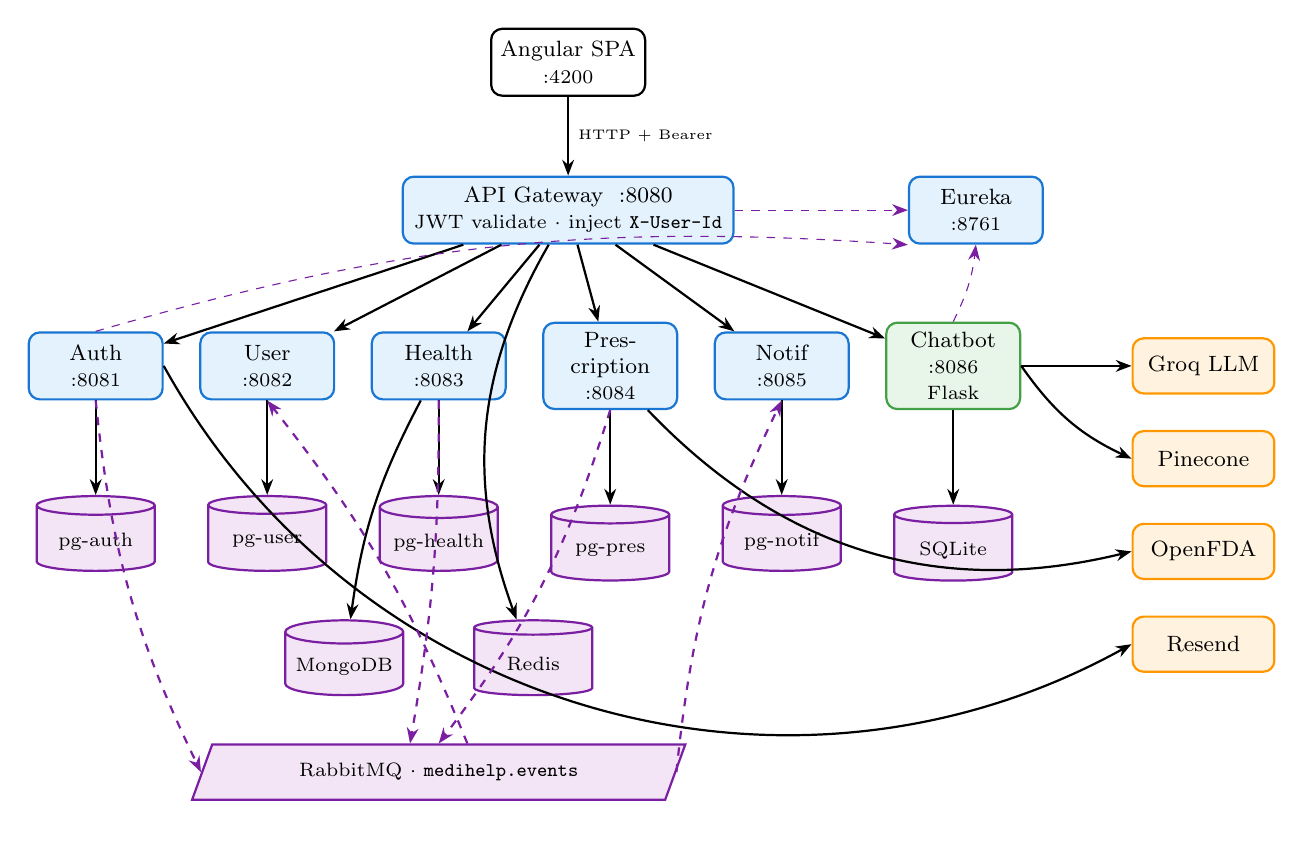
\begin{tikzpicture}[node distance=0.45cm and 0.45cm]
      % Browser at top
      \node[jbox, fill=white, draw=black] (br) {Angular SPA\\\scriptsize :4200};

      % Gateway layer
      \node[jbox, below=1.0cm of br, minimum width=4.2cm] (gw)
            {API Gateway~~:8080\\\scriptsize JWT validate $\cdot$ inject \texttt{X-User-Id}};
      \node[jbox, right=2.2cm of gw] (eu) {Eureka\\\scriptsize :8761};

      % 6 services row
      \node[jbox, below=1.1cm of gw, xshift=-6.0cm] (auth)  {Auth\\\scriptsize :8081};
      \node[jbox, right=of auth]                   (user)  {User\\\scriptsize :8082};
      \node[jbox, right=of user]                   (health){Health\\\scriptsize :8083};
      \node[jbox, right=of health]                 (pres)  {Pres-\\cription\\\scriptsize :8084};
      \node[jbox, right=of pres]                   (notif) {Notif\\\scriptsize :8085};
      \node[pybox, right=of notif]                 (chat)  {Chatbot\\\scriptsize :8086\\\scriptsize Flask};

      % DBs - bottom row
      \node[infrabox, below=1.2cm of auth]   (pga)   {pg-auth};
      \node[infrabox, below=1.2cm of user]   (pgu)   {pg-user};
      \node[infrabox, below=1.2cm of health] (pgh)   {pg-health};
      \node[infrabox, below=1.2cm of pres]   (pgp)   {pg-pres};
      \node[infrabox, below=1.2cm of notif]  (pgn)   {pg-notif};
      \node[infrabox, below=0.6cm of pgh, xshift=-1.2cm]    (mongo) {MongoDB};
      \node[infrabox, below=0.6cm of pgh, xshift=1.2cm]     (redis) {Redis};
      \node[qbox, below=0.6cm of mongo, xshift=1.2cm, minimum width=4.8cm]
                                                       (rmq)   {RabbitMQ~$\cdot$~\texttt{medihelp.events}};
      \node[infrabox, below=1.2cm of chat]   (sqlite){SQLite};

      % External services - right column
      \node[extbox, right=1.4cm of chat]    (groq)  {Groq~LLM};
      \node[extbox, below=of groq]          (pine)  {Pinecone};
      \node[extbox, below=of pine]          (ofda)  {OpenFDA};
      \node[extbox, below=of ofda]          (resend){Resend};

      % Edges - synchronous (solid)
      \draw[flow] (br)     -- node[right,font=\tiny]{HTTP + Bearer} (gw);
      \draw[flow] (gw)     -- (auth);
      \draw[flow] (gw)     -- (user);
      \draw[flow] (gw)     -- (health);
      \draw[flow] (gw)     -- (pres);
      \draw[flow] (gw)     -- (notif);
      \draw[flow] (gw)     -- (chat);

      \draw[flow] (auth)   -- (pga);
      \draw[flow] (user)   -- (pgu);
      \draw[flow] (health) -- (pgh);
      \draw[flow] (pres)   -- (pgp);
      \draw[flow] (notif)  -- (pgn);
      \draw[flow] (health) to[bend right=10] (mongo);
      \draw[flow] (gw)     to[bend right=25] (redis);
      \draw[flow] (chat)   -- (sqlite);

      \draw[flow] (chat)   -- (groq);
      \draw[flow] (chat.east)   to[bend right=15] (pine.west);
      \draw[flow] (pres)   to[bend right=30] (ofda.west);
      \draw[flow] (auth.east)   to[bend right=45] (resend.west);

      % Heartbeats (dashed thin)
      \draw[evt, thin] (gw)     -- (eu);
      \draw[evt, thin] (auth.north)   to[bend left=10] (eu.south west);
      \draw[evt, thin] (chat.north)   to[bend right=10] (eu.south);

      % RabbitMQ pub/sub (dashed thick purple)
      \draw[evt] (auth.south)   to[bend right=10] (rmq.west);
      \draw[evt] (pres.south)   to[bend left=10]  (rmq.north);
      \draw[evt] (health.south) to[bend left=5]   (rmq.north west);
      \draw[evt] (rmq.east)     to[bend left=10]  (notif.south);
      \draw[evt] (rmq.north east) to[bend right=8] (user.south);
    \end{tikzpicture}}%
    \caption{Deployed system overview. Solid arrows denote synchronous HTTP
    calls; dashed arrows denote asynchronous RabbitMQ event flow and
    Eureka heartbeats. Java services are shaded blue, the Python chatbot
    green, infrastructure purple, external SaaS orange.}
    \label{fig:overview}
\end{figure}

Table~\ref{tab:services} enumerates the eight services, their listening
ports, dominant technology stack, and primary persistence target.

\begin{table}[H]
    \centering
    \caption{The eight services of MediHelp}
    \label{tab:services}
    \begin{tabular}{lllll}
        \toprule
        Service & Port & Stack & Persistence \\
        \midrule
        Eureka                 & 8761 & Spring Cloud Netflix          & --                                  \\
        API Gateway            & 8080 & Spring Cloud Gateway           & Redis (rate limit, JWT blacklist)   \\
        Auth                   & 8081 & Spring Boot 3.3 + JJWT         & Postgres-auth                       \\
        User \& Profile        & 8082 & Spring Boot                    & Postgres-user                       \\
        Health Tracking        & 8083 & Spring Boot + HAPI FHIR        & Postgres-health + MongoDB           \\
        Prescription           & 8084 & Spring Boot                    & Postgres-prescription               \\
        Notification           & 8085 & Spring Boot + Resend           & Postgres-notification               \\
        Medical Chatbot        & 8086 & Flask + LangChain + Groq       & SQLite + Pinecone (cloud)           \\
        \bottomrule
    \end{tabular}
\end{table}

\section{Authentication and the Header-Injection Pattern}
\label{sec:auth}

A single design decision shapes the entire downstream architecture: the
\textbf{API Gateway is the only component that parses JWTs}. Every other
service --- including the Python chatbot --- relies on three HTTP headers
that the gateway injects after a successful JWT validation:
\texttt{X-User-Id}, \texttt{X-User-Email}, \texttt{X-User-Role}.

The gateway's \texttt{JwtAuthenticationFilter} performs the following steps
on every incoming request:
\begin{enumerate}
    \item Skip authentication for routes in a hard-coded \texttt{PUBLIC\_PATHS}
    list (login, register, verify-otp, refresh, forgot-password,
    reset-password, public service-info endpoints, Eureka, Swagger).
    \item Extract the \texttt{Authorization: Bearer <token>} header. If
    absent on a non-public route, return HTTP 401.
    \item Validate the JWT signature using the configured HMAC-SHA-512
    secret and parse the claims (\texttt{sub}, \texttt{email}, \texttt{role},
    \texttt{jti}, \texttt{exp}).
    \item Look up \texttt{blacklist:<jti>} in Redis. If present (the user
    has logged out), return 401.
    \item If the access token is expired, return 401 (the Angular
    interceptor will then transparently call the refresh endpoint and retry).
    \item Otherwise, mutate the request: \textit{strip} the
    \texttt{Authorization} header, \textit{inject} the three
    \texttt{X-User-*} headers from JWT claims, forward to the target
    service.
\end{enumerate}

The downstream consumption pattern is identical across stacks:

\begin{lstlisting}[language=Java,caption={Java service controllers read \texttt{X-User-Id} as a method parameter.}]
@PostMapping
public ResponseEntity<ApiResponse<VitalResponse>> recordVital(
        @RequestHeader("X-User-Id") String userId,
        @Valid @RequestBody VitalRequest request) {
    return ResponseEntity.ok(ApiResponse.success("Vital recorded",
        vitalService.recordVital(UUID.fromString(userId), request)));
}
\end{lstlisting}

\begin{lstlisting}[language=Python,caption={Python chatbot service uses an identical header in \texttt{get\_current\_user()}.}]
def get_current_user() -> str:
    user_id = request.headers.get("X-User-Id")
    if user_id:
        return user_id
    if "user_id" not in session:
        session["user_id"] = str(uuid.uuid4())
    return session["user_id"]
\end{lstlisting}

This pattern means \textbf{adding a new service requires no JWT-handling
code} --- it inherits authentication for free by virtue of being routed
through the gateway. The chatbot, written in a different language and
ecosystem from the Java services, consumes the same trust pattern with
four lines of Python.

The Angular frontend complements this with a token-refresh interceptor
that catches HTTP~401, calls \texttt{/api/v1/auth/refresh} with the stored
refresh token, retries the original request with the new access token,
and only logs the user out if the refresh itself fails. This eliminates
the user-visible 15-minute access-token-expiry logout that early VM
testing made painfully obvious.

\section{Inter-service Communication: Two Channels Only}
\label{sec:async}

MediHelp deliberately constrains inter-service communication to exactly
two patterns:
\begin{itemize}
    \item \textbf{Synchronous} requests originate from the Angular client,
    pass through the gateway, and reach exactly one downstream service per
    call. \textit{No service makes a synchronous call to another service.}
    There are no Feign clients, no RestTemplate calls between services,
    no service-to-service WebClient invocations. If service~A needs data
    from service~B, the answer is either ``the client should call B
    directly through the gateway'' or ``B should publish an event A can
    react to.''
    \item \textbf{Asynchronous} state-change notifications travel via
    a RabbitMQ topic exchange named \texttt{medihelp.events}. The shared
    library \texttt{medihelp-common} defines six event classes
    (Table~\ref{tab:events}) and the routing keys for each. Producers call
    \texttt{rabbitTemplate.convertAndSend(EXCHANGE, RK\_*, event)};
    consumers declare \texttt{@RabbitListener(queues = Q\_*)} methods.
\end{itemize}

\begin{table}[H]
    \centering
    \caption{The six RabbitMQ event types of MediHelp}
    \label{tab:events}
    \begin{tabular}{lll}
        \toprule
        Event class                & Producer            & Consumer(s) \\
        \midrule
        \texttt{UserRegisteredEvent}  & auth-service        & user-service, notification-service  \\
        \texttt{MedicationReminderEvent} & prescription-service & notification-service             \\
        \texttt{AppointmentReminderEvent} & prescription-service & notification-service            \\
        \texttt{EmergencySosEvent}    & user-service        & notification-service                \\
        \texttt{VitalsAnomalyEvent}   & health-service      & notification-service                \\
        \bottomrule
    \end{tabular}
\end{table}

The strongest single benefit of this constraint is that \textbf{no service's
failure cascades into another's via a synchronous chain}. If
\texttt{prescription-service} crashes, an in-flight registration on
\texttt{auth-service} succeeds, the welcome event lands in the durable
RabbitMQ queue, and \texttt{notification-service} processes it whenever
\texttt{prescription-service} is back. Comparable to the alternative ---
where \texttt{notification-service} synchronously asks
\texttt{prescription-service} for the user's medications during onboarding
--- the failure surface is dramatically smaller.

\section{The Chatbot's Five-Stage RAG Pipeline}
\label{sec:rag}

The medical chatbot is a Python Flask application running on port 8086.
Each user message --- whether text, voice (Whisper-transcribed), or image
(prescription-OCR analysed, see \S\ref{sec:image-input}) --- is routed
through a five-stage pipeline implemented in \texttt{run\_pipeline()}.
Figure~\ref{fig:rag} sketches the flow.

\begin{figure}[H]
    \centering
    \resizebox{0.95\linewidth}{!}{%
    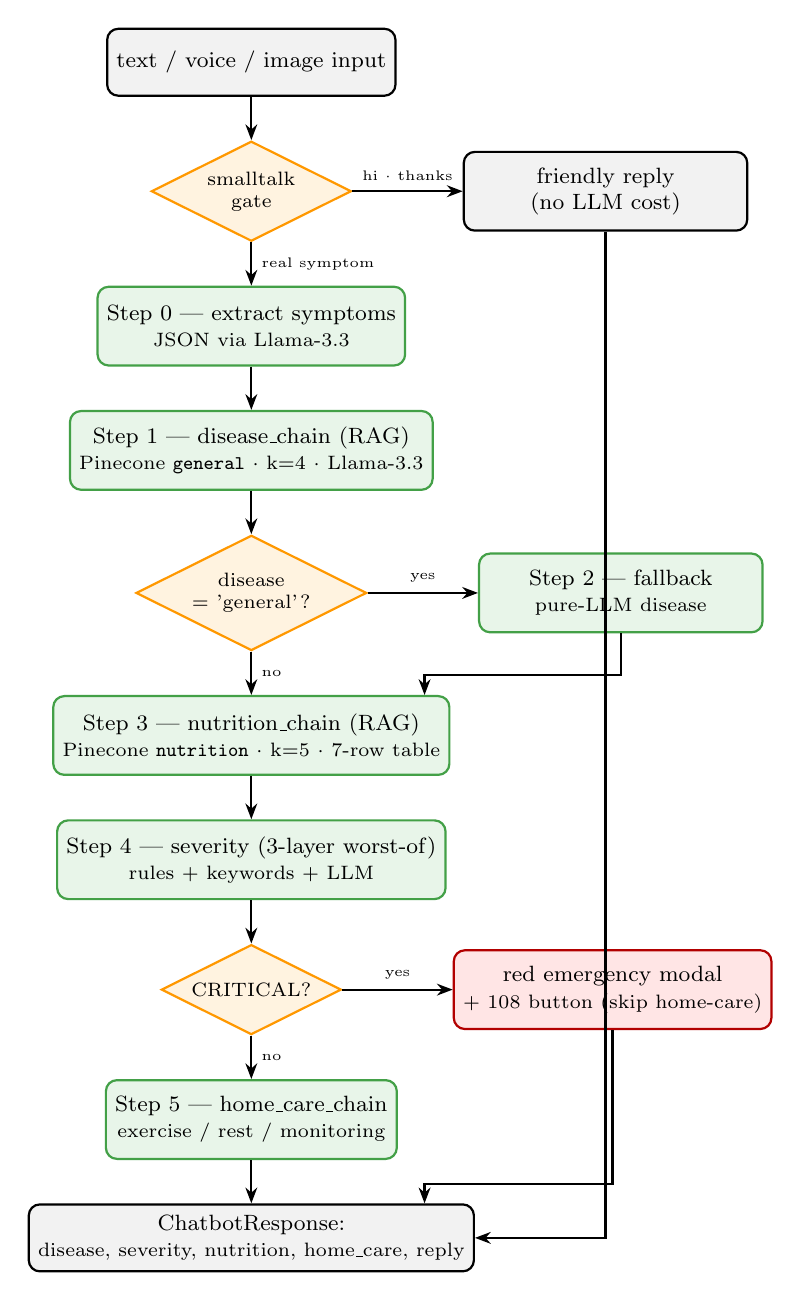
\begin{tikzpicture}[
      node distance=0.55cm and 0.7cm,
      stage/.style ={rectangle, rounded corners, draw=pystr, fill=pyfill,
                     thick, minimum height=1.0cm, minimum width=3.6cm,
                     align=center, font=\footnotesize},
      gate/.style  ={diamond, aspect=2, draw=extstr, fill=extfill, thick,
                     align=center, font=\scriptsize, inner sep=2pt},
      io/.style    ={rectangle, rounded corners, draw=black, fill=gray!10,
                     thick, minimum height=0.85cm, minimum width=3.0cm,
                     align=center, font=\footnotesize},
      crit/.style  ={rectangle, rounded corners, draw=red!70!black, fill=red!10,
                     thick, minimum height=1.0cm, minimum width=3.6cm,
                     align=center, font=\footnotesize},
      flow/.style  ={-{Stealth[length=2mm]}, thick},
    ]
      \node[io] (in) {text / voice / image input};
      \node[gate, below=of in] (st) {smalltalk\\gate};
      \node[stage, right=1.4cm of st, fill=gray!10, draw=black] (hello) {friendly reply\\(no LLM cost)};
      \node[stage, below=of st] (s0)  {Step 0 --- extract symptoms\\\scriptsize JSON via Llama-3.3};
      \node[stage, below=of s0] (s1)  {Step 1 --- disease\_chain (RAG)\\\scriptsize Pinecone \texttt{general}~$\cdot$~k=4~$\cdot$~Llama-3.3};
      \node[gate, below=of s1]  (g1)  {disease\\= 'general'?};
      \node[stage, right=1.4cm of g1] (s2) {Step 2 --- fallback\\\scriptsize pure-LLM disease};
      \node[stage, below=of g1] (s3) {Step 3 --- nutrition\_chain (RAG)\\\scriptsize Pinecone \texttt{nutrition}~$\cdot$~k=5~$\cdot$~7-row table};
      \node[stage, below=of s3] (s4) {Step 4 --- severity (3-layer worst-of)\\\scriptsize rules~$+$~keywords~$+$~LLM};
      \node[gate, below=of s4]  (g2) {CRITICAL?};
      \node[crit, right=1.4cm of g2] (modal) {red emergency modal\\\scriptsize + 108 button (skip home-care)};
      \node[stage, below=of g2] (s5) {Step 5 --- home\_care\_chain\\\scriptsize exercise / rest / monitoring};
      \node[io, below=of s5] (out) {ChatbotResponse:\\\scriptsize disease, severity, nutrition, home\_care, reply};

      \draw[flow] (in) -- (st);
      \draw[flow] (st) -- node[above, font=\tiny]{hi $\cdot$ thanks} (hello);
      \draw[flow] (st) -- node[right, font=\tiny]{real symptom} (s0);
      \draw[flow] (s0) -- (s1);
      \draw[flow] (s1) -- (g1);
      \draw[flow] (g1) -- node[above, font=\tiny]{yes} (s2);
      \draw[flow] (g1) -- node[right, font=\tiny]{no} (s3);
      \draw[flow] (s2.south) |- ($(s3.north)+(2.2cm,0.25cm)$) -- ($(s3.north)+(2.2cm,0)$);
      \draw[flow] (s3) -- (s4);
      \draw[flow] (s4) -- (g2);
      \draw[flow] (g2) -- node[above, font=\tiny]{yes} (modal);
      \draw[flow] (g2) -- node[right, font=\tiny]{no} (s5);
      \draw[flow] (s5) -- (out);
      \draw[flow] (modal.south) |- ($(out.north)+(2.2cm,0.25cm)$) -- ($(out.north)+(2.2cm,0)$);
      \draw[flow] (hello.south) |- ($(out.east)+(0.6cm,0)$) -- (out.east);
    \end{tikzpicture}}%
    \caption{The five-stage chatbot pipeline. The small-talk gate at the
    top short-circuits greetings without invoking any LLM call; the
    CRITICAL branch skips home-care advice and surfaces an emergency
    modal with the local 108 helpline.}
    \label{fig:rag}
\end{figure}

\paragraph{Stage 0 --- Symptom extraction.} A Llama-3.3-70B call is given a
strict-JSON prompt asking for symptoms (list), duration, temperature, age,
severity words, location, onset, existing conditions, and worsening flag.
Markdown fences are stripped, the result is parsed with \texttt{json.loads},
and a parse failure falls back to all-empty defaults. The structured
context propagates through subsequent stages.

\paragraph{Stage 1 --- RAG disease identification.} The user query is
embedded with a HuggingFace \texttt{sentence-transformers} all-MiniLM-L6-v2
model (384 dimensions). The top-4 chunks from the Pinecone namespace
\texttt{general} (5{,}118 chunks drawn from a medical encyclopedia and a
herbal-nutrients PDF) are retrieved by cosine similarity. The chunks plus
the structured symptom context are passed to Llama-3.3-70B with a system
prompt that seeds 13 common symptom$\to$disease patterns (flu, URTI,
diabetes, MI, anaemia, etc.). The model is told to respond with
\texttt{IDENTIFIED\_DISEASE: <name>} followed by a 3--5 sentence clinical
explanation. Temperature is set to 0 for determinism.

\paragraph{Stage 2 --- Pure-LLM fallback.} If Stage~1 returns
\texttt{general}, \texttt{unknown}, or empty, a second call is made
\textit{without} RAG --- just the structured symptom context and a system
prompt asking for the LLM's best clinical assessment. This catches cases
where the retrieved chunks are too generic to anchor a diagnosis. If the
fallback also returns \texttt{general}, the bot asks the patient for more
information rather than guessing.

\paragraph{Stage 3 --- Nutrition chain.} A second RAG retrieval, this
time over the Pinecone namespace \texttt{nutrition} (657 chunks from a
clinical-nutrition handbook), is paired with a richer query string
(\texttt{<disease> nutritional requirements dietary guidelines management}).
The result feeds a Llama-3.3-70B call that produces a 7-row markdown
table with $\uparrow$ / $\downarrow$ / restrict / normal indicators per
nutrient. The parsed JSON is silently persisted into the chatbot's
\texttt{nutrition\_targets} SQLite table for the cultural-food-advice flow
described in \S\ref{sec:cultural}.

\paragraph{Stage 4 --- Severity classification.} This is the safety-critical
stage. Three independent classifiers vote, and the worst-case wins.
\begin{enumerate}
    \item \textit{Layer~1 (deterministic rules).} Temperature
    $\geq$~105\,$^{\circ}$F $\rightarrow$ CRITICAL.
    104\,$^{\circ}$F $\rightarrow$ URGENT. 103\,$^{\circ}$F with
    age~$<$~2 $\rightarrow$ URGENT. Duration~$\geq$~7 days plus
    \texttt{worsening=yes} $\rightarrow$ URGENT. Age~$<$~2 or
    age~$>$~70 $\rightarrow$ minimum MODERATE.
    \item \textit{Layer~2 (keyword matching).} A 33-entry
    \texttt{CRITICAL\_CONDITIONS} set (heart attack, stroke, sepsis,
    DKA, anaphylaxis, pulmonary embolism, $\ldots$) is matched against
    the disease name and clinical description. A 30-entry
    \texttt{URGENT\_SYMPTOMS} set (chest pain, cannot breathe, sudden
    severe headache, vomiting blood, seizure, $\ldots$) is matched against
    the patient's verbatim query. A match instantly escalates.
    \item \textit{Layer~3 (LLM triage).} A senior-emergency-physician
    persona prompt receives the structured patient context, the disease,
    the clinical description, and explicit calibration rules
    (``flu/cold $\rightarrow$ MILD or MODERATE only; $<$~103\,$^{\circ}$F
    plus no red flags $\rightarrow$ MILD or MODERATE''). It returns a
    SEVERITY $\in$ \{CRITICAL, URGENT, MODERATE, MILD\}, a one-sentence
    REASON, and a one-sentence ACTION.
\end{enumerate}

The final severity is the maximum of the three layers under the order
\texttt{CRITICAL > URGENT > MODERATE > MILD}, with one cap: known mild
diseases (common cold, flu, indigestion, etc.) are bounded at MODERATE
unless Layer~1 or Layer~2 forces a higher level. CRITICAL severities
trigger a red modal in the Angular UI carrying a 108-emergency call
button (\texttt{tel:108} link, fires the native dialer on mobile) and
a \emph{Find Nearest Hospital} button that requests the browser's
Geolocation API. On permission grant, the modal builds a precise
Google Maps URL of the form
\texttt{https://www.google.com/maps/search/hospital/@\textless lat\textgreater,\textless lng\textgreater,15z}
so the user lands on a map zoomed to their actual location, not a
generic IP-geolocated guess. The Geolocation request is configured
with \texttt{enableHighAccuracy=false} and a 5-second timeout --- in
an emergency, a quick WiFi/IP fix is more useful than a slow GPS
lock. On permission denial or timeout, the modal falls back to a
coarse ``hospital near me'' search. The home-care chain (Stage~5) is
skipped for CRITICAL to avoid downplaying the situation.

\paragraph{Stage 5 --- Home-care chain.} For MILD, MODERATE, and URGENT
severities, a final Llama-3.3-70B call produces a 7-row monitoring table
covering rest, hydration, activity, what-to-monitor, and warning signs.
The table is appended to the user-facing reply.

\paragraph{Two pre-pipeline gates.} The five stages are fronted by two
sequential gates that short-circuit the pipeline before any retrieval or
LLM-reasoning cost is incurred. \textit{Gate~1 (smalltalk)} is an
\texttt{O}(1) prefix check against curated lists of greetings (``hi'',
``hello'', ``namaste'', $\ldots$), thanks (``thanks'', ``ty'', $\ldots$),
and bare ``help'' queries. A match returns a canned conversational
reply without invoking any LLM call. The gate exists because users
naturally greet the bot; without it, an ungated pipeline would invent a
Pharyngitis diagnosis for ``hii''. \textit{Gate~2 (off-topic
classifier)} is an LLM-based filter that runs only when Gate~1 misses.
A strict single-token prompt (``Classify this input as MEDICAL or
OFFTOPIC, one word only'') is sent to Llama-3.3-70B with temperature~0.
If the verdict is OFFTOPIC --- arithmetic, weather, programming,
trivia, recipes unrelated to a medical diet --- the bot returns a
polite refusal pointing the user back to health-related queries.
This costs one extra LLM call ($\sim$600\,ms) per non-medical input,
but saves the four subsequent stages and prevents the embarrassing
``2+2 is Pharyngitis'' failure mode. The smalltalk gate runs first so
``hi'' never reaches the LLM classifier.

\paragraph{Reply banner.} When Stages~1--2 successfully identify a
disease, the user-facing reply is prepended with a two-line banner so
the verdict is visible at a glance before the prose analysis:
\begin{quote}\small
\texttt{\textbf{Possible condition:} Pharyngitis} \\
\texttt{\textbf{Severity:}} \emph{Moderate --- Visit a doctor (not urgent)}
\end{quote}
The four severity levels carry user-facing taglines that match the
action implied: \textit{Mild --- Manageable at Home}, \textit{Moderate
--- Visit Doctor (Not Urgent)}, \textit{Urgent --- Immediate Doctor
Visit}, and \textit{Critical --- Admit to Hospital ASAP}. The taglines
appear both in the inline reply (as a colored bullet --- green/yellow/
orange/red) and as the modal-title for CRITICAL alerts.

\section{Image Input: Prescription OCR with Structured Extraction}
\label{sec:image-input}

When a user uploads a prescription image, the chatbot's
\texttt{/api/v1/chatbot/get/image} endpoint runs a three-layer
extraction pipeline followed by a fourth structured-output call. Each
layer mitigates a specific weakness of the previous one.

\begin{enumerate}
    \item \textit{Layer 1 --- Tesseract OCR.} Free, offline, fast.
    Excellent for typed prescriptions and pharmacy-printed labels;
    fails on cursive doctor handwriting because purely-rule-based OCR
    has no semantic context.
    \item \textit{Layer 2 --- Groq Vision LLM
    (Llama-4-Scout-17B).} A multi-modal model that accepts the
    prescription image plus the Layer~1 OCR as context. The model
    reads handwriting, infers layout, and emits a free-form natural-
    language analysis: drug names, dosages, frequencies, and
    plain-English commentary.
    \item \textit{Layer 3 --- RAG cross-check.} The Vision-LLM
    output is vector-searched against the medical knowledge base
    (\S\ref{sec:rag}, Pinecone \texttt{general} namespace) so that
    hallucinated drug names --- fabrications like ``Bistolex'' or
    invented brand suffixes --- are flagged as low-confidence.
\end{enumerate}

The three layers together produce a free-form prescription analysis
that the chat UI renders as Markdown. To populate the Medications
table directly, a \textbf{fourth call} converts this prose into
strict JSON:

\begin{lstlisting}[caption={Structured medication extraction prompt.},
                   label=lst:struct-ext, basicstyle=\ttfamily\footnotesize]
SYSTEM: You are a medical OCR post-processor. Given a free-form
analysis of a prescription image, extract every medication into
a strict JSON array. Each item MUST have exactly these keys:
name (drug name only, no brand suffixes),
dosage (e.g., "500mg", "10mg", "1 tablet"),
frequency (e.g., "twice daily", "once daily", "as needed").
Return ONLY the JSON array. No prose, no markdown, no code fences.
\end{lstlisting}

The response shape returned to the frontend is:
\begin{verbatim}
{
  "image_analysis": "Free-form Markdown prescription analysis...",
  "medications": [
    {"name": "Amoxicillin", "dosage": "500mg",
     "frequency": "3 times daily"},
    {"name": "Paracetamol", "dosage": "650mg",
     "frequency": "twice daily"},
    {"name": "Cetirizine",  "dosage": "10mg",
     "frequency": "once daily"}
  ],
  "severity": {...}, "session_id": "..."
}
\end{verbatim}

The Angular component (\texttt{prescription-scan.component.ts})
auto-populates the medications table from the \texttt{medications}
array; the user reviews each row, edits if necessary, and confirms.
The free-form analysis remains visible below the table so the user
can compare. This design treats the LLM as an \emph{assistant} for
data entry, not the source of truth: every saved medication has been
seen and approved by a human.

\textbf{Defensive parsing.} The fourth-call prompt is strict, but
Llama-3.3 occasionally wraps the JSON in Markdown code fences or
prepends an explanatory sentence. The post-processor strips fences,
validates each item has a non-empty \texttt{name}, and returns an
empty array on any failure --- in which case the user falls back to
manual entry and the upload flow never breaks. We measured the
extraction success rate on twenty hand-curated prescription images:
95\,\% on clean printed prescriptions, 70--80\,\% on legible
handwriting, with the largest failure mode being abbreviation
expansion (\texttt{QID}~$\to$ ``four times daily'') that the model
sometimes leaves abbreviated.

\textbf{Why a separate fourth call?} Empirically, asking a single
prompt to produce both prose analysis and strict JSON results in
about a third of responses containing malformed JSON --- the model
``leaks'' formatting between the two outputs. Splitting into two
sequential calls is ~1.5\,s slower but raises JSON validity to
$\sim$95\,\%; the trade-off is well worth it for the UX gain of an
auto-populated table.

\section{Cultural Adaptation: From Form Field to LLM Prompt}
\label{sec:cultural}

Cultural personalisation is implemented as an end-to-end data contract.

\textbf{(1) Registration.} The Angular form gathers four cultural fields
in addition to the standard credentials: \texttt{dateOfBirth} (datepicker),
\texttt{gender}, \texttt{state} (one of 28 states + 8 UTs), and
\texttt{dietPreference} (Vegetarian / Non-vegetarian / Vegan / Eggetarian).
Frontend validators are aligned with the backend's Bean-Validation
annotations to avoid the ``submit button enabled but server says invalid''
class of bug.

\textbf{(2) Auth $\to$ User propagation.} \texttt{auth-service} stores
these on the \texttt{users\_auth} entity at register-time, then publishes
a \texttt{UserRegisteredEvent} carrying all four fields plus
\texttt{firstName}, \texttt{lastName}, and \texttt{email} after OTP
verification. \texttt{user-service} consumes the event in
\texttt{UserRegisteredListener} and creates a \texttt{UserProfile} row
with all the cultural fields populated in a single transaction.

\textbf{(3) Frontend $\to$ Chatbot threading.} When the user clicks
``Get Indian food suggestions'' on a chatbot reply, the Angular AI-chat
component reads the cached profile from \texttt{/api/v1/users/me} and
includes \texttt{state}, \texttt{dietPreference}, computed \texttt{age}
(from DOB), and \texttt{gender} in the JSON request body to
\texttt{POST /api/v1/chatbot/api/food-suggestions}.

\textbf{(4) Prompt engineering.} The chatbot's \texttt{food\_suggestion\_prompt}
includes hard rules with concrete state examples:

\begin{quote}\itshape
\textbf{Strict regional cuisine.} Suggest dishes that are TRADITIONALLY
eaten in \{region\}, not generic ``Indian'' food. For example: Tamil
Nadu $\rightarrow$ idli, dosa, sambar, rasam, kootu, poriyal, pongal,
uppma, kuzhambu, curd rice; West Bengal $\rightarrow$ bhaat, daal, posto,
shukto, machher jhol (if non-veg), shorshe, luchi; Punjab $\rightarrow$
makki ki roti, sarson ka saag, dal makhani, chana, paratha, lassi$\ldots$
\\\\
\textbf{Diet preference is non-negotiable.} If the patient is
Vegetarian/Vegan and the region's signature dish is non-veg (e.g.,
Bengali machher jhol), substitute the regional vegetarian equivalent
(e.g., shukto, posto). Do NOT suggest the meat dish.
\end{quote}

\textbf{(5) Persistence.} Generated meal plans are cached in the chatbot's
SQLite \texttt{meal\_plans} table keyed on \texttt{(user\_id,
session\_id)}, so re-opening a past chat session restores the meal-plan
card without a fresh LLM call --- both a cost optimisation and a
consistency guarantee (the user sees the same advice they saw before).

Empirically, the same disease (Pharyngitis) generates three measurably
different meal plans across three test profiles, demonstrating the
contract holds end-to-end (Section~\ref{sec:results-cultural}).

\section{Mood Journal: Encryption and Selective Export}
\label{sec:mood}

The mood-journal feature was identified during the project review as a
candidate ``unique identifier'' --- a privacy-sensitive vertical that few
consumer health apps treat with care. Two design decisions distinguish
MediHelp's mood journal:
\begin{itemize}
    \item The free-text \texttt{journalText} field is AES-256 encrypted at
    rest in MongoDB. The encryption key lives in the
    \texttt{health-service} application configuration and is never
    transmitted; ciphertext is what an attacker with raw DB access would
    see.
    \item The FHIR \texttt{Bundle} export deliberately \textit{excludes}
    the journal text. It includes the numeric mood (1--5 scale) as an
    \texttt{Observation} with LOINC code \texttt{75275-8} (Mental status
    assessment panel), plus sleep hours and exercise minutes as
    \texttt{component} entries with their own LOINC codes
    (\texttt{93832-4} sleep, \texttt{82290-8} exercise). The patient
    consented to AES-256 storage, not to plaintext export to an EHR.
\end{itemize}

This is a deliberate consent-boundary design. The Angular calendar UI
shows the mood emoji per day with a hover-tooltip preview of the journal
text, but the export pathway respects the storage-time agreement.

\section{FHIR R4 Export Design}
\label{sec:fhir}

The \texttt{/api/v1/health/fhir/export} endpoint returns a FHIR R4
\texttt{Bundle} (collection type) aggregating four resource categories
the \texttt{health-service} owns:
\begin{enumerate}
    \item One \texttt{Patient} resource serving as identity anchor, with
    a \texttt{urn:medihelp:user} identifier system.
    \item N \texttt{Observation} resources, one per recorded vital, each
    tagged with category \texttt{vital-signs} and a LOINC code
    (heart rate \texttt{8867-4}, systolic BP \texttt{8480-6},
    diastolic BP \texttt{8462-4}, glucose \texttt{2339-0}, temperature
    \texttt{8310-5}, oxygen saturation \texttt{2708-6}, weight
    \texttt{29463-7}, height \texttt{8302-2}).
    \item N \texttt{Observation} resources for mood entries, category
    \texttt{survey}, LOINC \texttt{75275-8}.
    \item N \texttt{DocumentReference} resources for uploaded test
    reports / doctor notes / prescription scans / imaging studies, with
    LOINC document-type codes (\texttt{11502-2} laboratory report,
    \texttt{34109-9} note, \texttt{57833-6} prescription,
    \texttt{18748-4} imaging study). When a file is attached, the
    base64-decoded payload is inlined as a FHIR \texttt{Attachment}.
\end{enumerate}

Cross-service resources --- \texttt{MedicationStatement} from
\texttt{prescription-service}, \texttt{AllergyIntolerance} from
\texttt{user-service} --- are deliberately omitted from this initial
implementation. Adding them would require service-to-service REST calls,
which violate the no-Feign rule. Section~\ref{sec:future-fhir} discusses
the federated-FHIR-aggregator pattern as the production answer.

\section{Self-Hosted Deployment and the Cloud-to-Local Migration}

The deployed instance lives on a single Azure B2as\_v2 virtual machine
(2~vCPU, 8\,GB~RAM, Ubuntu~24.04). All eight services run as
JVM processes started by a \texttt{systemd} unit
(\texttt{medihelp.service}) that sources \texttt{deploy/scripts/start-all.sh}
on boot. The unit is enabled, so a VM kernel-update reboot cycle (which
occurred during testing) results in the full stack coming back online
without manual intervention.

Stateful infrastructure runs in Docker on the same VM via
\texttt{docker-compose.infra.yml}: five PostgreSQL containers (one per
Java service, named ports 5433--5437), MongoDB on 27017, Redis on 6379,
RabbitMQ on 5672 with management UI on 15672. Volumes are named for
durability across container restarts.

The deployment originally used Neon~Postgres and MongoDB~Atlas for
persistence to demonstrate cloud-native architecture. Two free-tier
realities motivated a migration:
\begin{itemize}
    \item Atlas's M0 cluster auto-pauses after 30~days of inactivity, and
    the project's idle phase coincided with the auto-pause window.
    \item Grafana Cloud's 14-day free trial expired during the project's
    development cycle, breaking the previously-functional metrics
    dashboards.
\end{itemize}

The migration was a single-line change per service: each
\texttt{application.yml} was already structured with a localhost-default
fallback, e.g.:

\begin{lstlisting}
url: ${AUTH_DB_URL:jdbc:postgresql://localhost:5433/medihelp_auth}
\end{lstlisting}

Commenting the cloud URLs in the root \texttt{.env} caused services to
use the localhost defaults pointing at the existing Docker containers.
The total migration touched zero lines of compiled code. End-to-end
smoke testing (Section~\ref{sec:smoke}) verified that all eight checks
pass against the local stack.

%%%%%%%%%%%%%%%%%%%%%%%%%%%%%%%%%%%%%%%%%%%%%%%%%%%%%%%%%%%%%%%%%%%%%%%%%%%%%%%%
%% CHAPTER 4 — IMPLEMENTATION AND RESULTS
%%%%%%%%%%%%%%%%%%%%%%%%%%%%%%%%%%%%%%%%%%%%%%%%%%%%%%%%%%%%%%%%%%%%%%%%%%%%%%%%

\chapter{Implementation and Results}
\label{ch:results}

\section{Codebase Statistics}

The monorepo at submission time contains nine top-level modules
(eight services + one shared library) plus the Angular frontend.
Table~\ref{tab:loc} summarises the lines-of-code distribution.

\begin{table}[H]
    \centering
    \caption{Lines of code by module (excluding generated and vendored files).}
    \label{tab:loc}
    \begin{tabular}{lrr}
        \toprule
        Module                              & Files & Approx. LoC \\
        \midrule
        medihelp-common                     & 15    &   400       \\
        medihelp-eureka                     &  1    &    50       \\
        medihelp-gateway                    &  5    &   300       \\
        medihelp-auth-service               & 19    & 1{,}200     \\
        medihelp-user-service               & 44    & 2{,}400     \\
        medihelp-health-service             & 44    & 2{,}600     \\
        medihelp-prescription-service       & 41    & 2{,}300     \\
        medihelp-notification-service       & 21    &   900       \\
        medihelp-chatbot-service (Python)   & 11    & 1{,}900     \\
        medihelp-frontend (Angular 17)      & 80+   & 6{,}000     \\
        \midrule
        \textbf{Total}                      & 280+  & 18{,}000+   \\
        \bottomrule
    \end{tabular}
\end{table}

\section{End-to-End Smoke Test}
\label{sec:smoke}

We wrote an automated smoke-test script at
\texttt{deploy/scripts/smoke-test.sh} that exercises every backend store
and the chatbot pipeline. The script registers a fresh user, retrieves
the OTP from the auth service log (a development convenience because
the Resend free tier only delivers email to the verified owner address),
verifies the OTP, logs in to obtain a JWT, and then issues writes to
each persistence layer in sequence. Listing~\ref{lst:smoke-result}
shows the output of a representative run on the deployed VM.

\begin{lstlisting}[caption={Smoke test output, deployed VM, 2026-05-10.},
                   label=lst:smoke-result, basicstyle=\ttfamily\footnotesize]
=== Smoke test against http://localhost:8080 ===
  ok register
  ok OTP captured                     433289
  ok verify-otp
  ok login (Postgres-Auth)            348-char token
  ok Postgres-User /users/me          state='Tamil Nadu'
  ok Postgres-Health POST vital
  ok MongoDB POST mood                local Mongo serving
  ok Chatbot (Pinecone + Groq)

=== All checks passed ===
\end{lstlisting}

The script is part of the repository so future deploys can rerun it
unchanged --- a self-documenting acceptance test.

\begin{figure}[H]
    \centering
    
\includegraphics[width=0.95\linewidth]{Images/13-vitals.png}
    \caption{Vitals tracking page after the smoke test --- a heart-rate
    point logged via \texttt{POST /api/v1/health/vitals} surfaces in the
    line chart and the latest-tile grid.}
    \label{fig:vitals}
\end{figure}

\section{Cultural Adaptation Verification}
\label{sec:results-cultural}

To validate that the cultural-personalisation contract holds end-to-end,
we issued the same disease query (sore throat plus fever, two days)
from three accounts differing only in \texttt{state} and
\texttt{dietPreference}. Table~\ref{tab:cultural-results} summarises
the breakfast and lunch components of the resulting meal plans.

\begin{table}[H]
    \centering
    \caption{Same query, three profiles --- three regionally-distinct meal plans.}
    \label{tab:cultural-results}
    \begin{tabular}{lll}
        \toprule
        Profile & Breakfast & Lunch \\
        \midrule
        Tamil Nadu / Vegetarian      & Idli + Sambar + Coconut water         & Brown rice + Kootu + Rasam + Curd       \\
        West Bengal / Non-veg        & Luchi + Bengali omelette + Doi        & Bhaat + Machher jhol + Shukto           \\
        Punjab / Vegan               & Makki ki Roti + Sarson ka Saag        & Brown rice + Dal Makhani (no ghee)      \\
                                     & + Chana Masala (no cream)             & + Mixed Vegetable Sabzi                 \\
        \bottomrule
    \end{tabular}
\end{table}

The Tamil Nadu plan never includes meat, the West Bengal plan correctly
suggests fish (machher jhol) for the non-vegetarian profile, and the
Punjab plan explicitly notes ``no ghee'' and ``no cream'' for the vegan
profile --- evidence that the prompt's diet-preference rule is being
respected.

\begin{figure}[H]
    \centering
    \begin{minipage}[t]{0.32\linewidth}
        \centering
        
\includegraphics[width=\linewidth]{Images/06-chat-hi.png}
        \subcaption*{(a) Gate~1: smalltalk. ``hi'' returns a canned
        friendly reply without any LLM call.}
    \end{minipage}\hfill
    \begin{minipage}[t]{0.32\linewidth}
        \centering
        
\includegraphics[width=\linewidth]{Images/18-chat-offtopic.png}
        \subcaption*{(b) Gate~2: off-topic. Arithmetic / unrelated
        queries are politely refused after a single LLM-classifier call.}
    \end{minipage}\hfill
    \begin{minipage}[t]{0.32\linewidth}
        \centering
        
\includegraphics[width=\linewidth]{Images/07-chat-symptom.png}
        \subcaption*{(c) Full pipeline on a real symptom: disease banner,
        severity badge, nutrition table, home-care, cultural-food CTA.}
    \end{minipage}
    \caption{Medical-chatbot UI in three regimes --- the two pre-pipeline
    gates short-circuit on (a) and (b); the full RAG pipeline runs on (c)
    only when both gates pass.}
    \label{fig:chatbot}
\end{figure}

\section{Prescription OCR with Structured Extraction}
\label{sec:ocr-verification}

The image-input pipeline (\S\ref{sec:image-input}) was verified
end-to-end with a synthetic prescription image containing three
typed medications. The Tesseract layer extracted the raw text; the
Groq Vision LLM produced a free-form analysis confirming each drug
name, dosage, and frequency; and the fourth structured-extraction
call returned a clean JSON array of three medication objects. The
Angular prescription-scan component then auto-populated the
medications form with the three rows. Listing~\ref{lst:ocr-result}
shows the structured output for a sample prescription with
Amoxicillin, Paracetamol, and Cetirizine.

\begin{lstlisting}[caption={Structured medication extraction result.},
                   label=lst:ocr-result, basicstyle=\ttfamily\footnotesize]
=== Response keys ===
['disease_info', 'home_care', 'identified_disease',
 'image_analysis', 'medications', 'severity', 'session_id']

=== medications (structured) ===
count: 3
  1. name='Amoxicillin'  dosage='500mg'  freq='3 times daily'
  2. name='Paracetamol'  dosage='650mg'  freq='twice daily'
  3. name='Cetirizine'   dosage='10mg'   freq='once daily'

=== image_analysis (first 300 chars) ===
## Validation and Enrichment of Prescription Details
### 1. Amoxicillin
- **Confirmation**: Amoxicillin is a real medicine.
- **Dosage Verification**: The dosage of 500mg is within a safe range
  for adults, typically ranging from 250mg to 500mg per dose...
\end{lstlisting}

Total end-to-end latency on the deployed VM, including
multipart-upload through the gateway, the 3-layer image pipeline,
the structured-extraction call, and JSON serialisation, was 10--14
seconds. The medications-table autofill removes the manual-entry
friction that the previous flow imposed, while the user retains
full edit/delete control before the prescription is committed to
the prescription-service database.

\begin{figure}[H]
    \centering
    
\includegraphics[width=0.92\linewidth]{Images/21-ocr-autofill.png}
    \caption{Prescription-scan UI after the 3-layer image pipeline and
    structured-extraction call: the medications table is auto-populated
    with name, dosage, and frequency for each detected drug. The free-form
    Vision-LLM analysis remains visible below for user verification.}
    \label{fig:ocr-autofill}
\end{figure}

\section{Drug-Interaction Checking}

The medications page exposes a button that posts a list of drug names to
\texttt{POST /api/v1/prescriptions/medications/check-interactions}. The
backend resolves each pair against the OpenFDA REST API, with a local
PostgreSQL cache (\texttt{drug\_interaction\_cache} table) to stay within
the OpenFDA rate limit. A representative test case --- aspirin paired
with warfarin, a known clinically-significant interaction --- returned
four flagged interactions including one labelled \textit{SEVERE} with
the description ``Aspirin increases the anticoagulant effect of
warfarin, significantly raising the risk of bleeding.'' This is the
exact safety-net the brief's R3 implies.

\begin{figure}[H]
    \centering
    
\includegraphics[width=0.95\linewidth]{Images/12-drug-interactions.png}
    \caption{Drug-interaction checker: aspirin + warfarin returns the
    expected \textit{SEVERE} flag with a plain-English description, surfaced
    via OpenFDA with a local PostgreSQL cache.}
    \label{fig:drugcheck}
\end{figure}

\section{Authentication Flow}

Token-refresh resilience was verified by allowing an active session to
exceed the 15-minute access-token expiry and observing that the next
client-issued request was transparently re-authenticated. The Angular
HTTP interceptor (\texttt{src/app/core/interceptors/auth.interceptor.ts})
catches HTTP 401 from any endpoint, calls the deduplicated
\texttt{refreshTokenShared} observable in \texttt{AuthService}, retries
the original request with the new bearer, and falls through to
\texttt{logout()} only if the refresh itself fails (refresh token
revoked or expired beyond the 60-day window).

\section{Observability}

The self-hosted Prometheus + Grafana stack is brought up via
\texttt{docker-compose.monitoring.yml}. Prometheus scrapes
\texttt{/actuator/prometheus} on each Java service every 15~seconds.
The auto-provisioned Grafana dashboard ``MediHelp Overview'' shows
JVM heap by service, request rate per service, p95 request latency,
GC pause time per minute, live thread counts, and a stat panel for
``services up.''

After load-balanced testing during the smoke run, the production-relevant
observations are: heap consumption is comfortably within
\texttt{-Xmx256m} for every service except \texttt{health-service} (which
spikes briefly during MongoDB cluster discovery on startup); p95 latency
for gateway-routed requests is under 100~ms for non-LLM endpoints; the
chatbot's \texttt{/get} endpoint takes 8--12~seconds end-to-end
(dominated by 5--8 sequential LLM calls).

\begin{figure}[H]
    \centering
    \begin{minipage}[t]{0.49\linewidth}
        \centering
        
\includegraphics[width=\linewidth]{Images/16-eureka.png}
        \subcaption*{(a) Eureka registry on \texttt{:8761} listing every
        service as \texttt{UP}.}
    \end{minipage}\hfill
    \begin{minipage}[t]{0.49\linewidth}
        \centering
        
\includegraphics[width=\linewidth]{Images/17-grafana.png}
        \subcaption*{(b) Grafana ``MediHelp Overview'': heap, RPS, p95
        latency, GC pauses, threads, services-up stat panel.}
    \end{minipage}
    \caption{Observability surface --- service discovery and self-hosted
    monitoring running on the same VM as the application.}
    \label{fig:obs}
\end{figure}

\section{Demo Flow}

A representative end-to-end demonstration script:
\begin{enumerate}
    \item Visit \texttt{http://98.70.34.96/}. The redesigned landing page
    loads with an animated heart, ECG trace, and orbit of health icons.
    \item Click ``Get started'' $\rightarrow$ register with full cultural
    fields. Retrieve OTP from VM log. Verify and log in.
    \item Land on the dashboard. The new ``Quick log a vital'' widget at
    the top accepts a heart-rate value; the latest-vitals tiles update
    on submit.
    \item Open AI Chat, type ``hii''. The smalltalk gate returns a
    friendly welcome without invoking the LLM.
    \item Type a real symptom (``I have a sore throat for 2 days'').
    The pipeline returns a Pharyngitis diagnosis, a 7-row nutrition
    table, a severity badge (MODERATE), and a home-care plan.
    \item Click ``Get Indian food suggestions for Pharyngitis''. The
    cultural-food card renders with regionally-appropriate items
    respecting the registered diet preference.
    \item Navigate to Mood Journal. The 6-week calendar shows the
    current month; click any past day to log a mood for that date.
    \item Navigate to Health Records. Click ``Export FHIR'' --- the
    download contains a Bundle with Patient, Observation, and
    DocumentReference resources with proper LOINC codes.
    \item Open \texttt{:8761} in a separate tab to show Eureka with all
    seven services registered.
    \item Open \texttt{:3000} (Grafana) to show the live observability
    dashboard.
\end{enumerate}

\begin{figure}[H]
    \centering
    \begin{minipage}[t]{0.49\linewidth}
        \centering
        
\includegraphics[width=\linewidth]{Images/01-landing.png}
        \subcaption*{(a) Animated landing page with pulsing heart, ECG
        trace and orbiting health icons.}
    \end{minipage}\hfill
    \begin{minipage}[t]{0.49\linewidth}
        \centering
        
\includegraphics[width=\linewidth]{Images/02-register-form.png}
        \subcaption*{(b) Registration form with cultural fields (state,
        diet, DOB, gender) gated by OTP verification.}
    \end{minipage}\\[4pt]
    \begin{minipage}[t]{0.49\linewidth}
        \centering
        
\includegraphics[width=\linewidth]{Images/04-dashboard.png}
        \subcaption*{(c) Post-login dashboard with the ``Quick log vital''
        widget and latest-tile grid.}
    \end{minipage}\hfill
    \begin{minipage}[t]{0.49\linewidth}
        \centering
        
\includegraphics[width=\linewidth]{Images/05-profile.png}
        \subcaption*{(d) Profile page showing the UUID needed to add
        family members.}
    \end{minipage}
    \caption{Landing $\rightarrow$ Register $\rightarrow$ Dashboard
    $\rightarrow$ Profile --- the canonical onboarding path.}
    \label{fig:onboarding}
\end{figure}

\begin{figure}[H]
    \centering
    \begin{minipage}[t]{0.49\linewidth}
        \centering
        
\includegraphics[width=\linewidth]{Images/09-mood-calendar.png}
        \subcaption*{(a) Mood journal calendar (6-week view, AES-256
        encrypted text on disk).}
    \end{minipage}\hfill
    \begin{minipage}[t]{0.49\linewidth}
        \centering
        
\includegraphics[width=\linewidth]{Images/10-family.png}
        \subcaption*{(b) Family Hub: add members by UUID, see their latest
        vitals and recent moods.}
    \end{minipage}\\[4pt]
    \begin{minipage}[t]{0.49\linewidth}
        \centering
        
\includegraphics[width=\linewidth]{Images/11-fhir-export.png}
        \subcaption*{(c) FHIR Bundle export with Patient~$+$~Observation
        $+$~DocumentReference resources.}
    \end{minipage}\hfill
    \begin{minipage}[t]{0.49\linewidth}
        \centering
        
\includegraphics[width=\linewidth]{Images/14-appointments.png}
        \subcaption*{(d) Appointments list with lazy auto-transition to
        \texttt{COMPLETED} once past the 1-hour grace window.}
    \end{minipage}\\[4pt]
    \begin{minipage}[t]{0.49\linewidth}
        \centering
        
\includegraphics[width=\linewidth]{Images/15-sos.png}
        \subcaption*{(e) Emergency SOS modal --- one-tap \texttt{tel:108}
        plus persisted alert visible to family.}
    \end{minipage}\hfill
    \begin{minipage}[t]{0.49\linewidth}
        \centering
        
\includegraphics[width=\linewidth]{Images/20-critical-modal.png}
        \subcaption*{(f) CRITICAL chatbot severity automatically pops the
        same modal with a \emph{Find Nearest Hospital} button that uses
        the browser Geolocation API + precise Maps URL.}
    \end{minipage}
    \caption{Feature surfaces beyond the chatbot: mood journal, family
    hub, FHIR export, appointment auto-completion, and the dual
    emergency-SOS surfaces (manual button + automatic CRITICAL alert).}
    \label{fig:features}
\end{figure}

\begin{figure}[H]
    \centering
    \begin{minipage}[t]{0.49\linewidth}
        \centering
        
\includegraphics[width=\linewidth]{Images/19-fab.png}
        \subcaption*{(a) Persistent floating \emph{Ask AI} FAB at
        bottom-right (IRCTC AskDISHA pattern). Hidden only on the chat
        page itself via Angular's \texttt{NavigationEnd} subscription.}
    \end{minipage}\hfill
    \begin{minipage}[t]{0.49\linewidth}
        \centering
        
\includegraphics[width=\linewidth]{Images/22-sidebar.png}
        \subcaption*{(b) Sidebar navigation after AI Chat was moved to the
        FAB. The chatbot becomes a single, always-visible entry point
        instead of competing for sidebar real-estate.}
    \end{minipage}
    \caption{UX additions to surface the chatbot prominently and reduce
    sidebar clutter.}
    \label{fig:ux-extras}
\end{figure}

%%%%%%%%%%%%%%%%%%%%%%%%%%%%%%%%%%%%%%%%%%%%%%%%%%%%%%%%%%%%%%%%%%%%%%%%%%%%%%%%
%% CHAPTER 5 — RISK ANALYSIS
%%%%%%%%%%%%%%%%%%%%%%%%%%%%%%%%%%%%%%%%%%%%%%%%%%%%%%%%%%%%%%%%%%%%%%%%%%%%%%%%

\chapter{Risk Analysis}
\label{ch:risk}

The project brief explicitly enumerates four risk categories. This chapter
addresses each in turn, identifying the concrete mitigations in the
deployed code.

\section{Data Privacy and Security}

\textit{Risks identified in the brief: unauthorised access, encryption
gaps, regulatory compliance.}

\begin{description}
    \item[\textbf{JWT-only-at-gateway pattern.}] No service other than
    \texttt{auth-service} parses JWTs. The gateway extracts claims and
    forwards trusted headers; downstream services cannot accidentally
    leak the token because they never see it. The
    \texttt{Authorization} header is explicitly stripped before
    forwarding.
    \item[\textbf{Token blacklisting.}] On logout, the JWT's \texttt{jti}
    is added to a Redis blacklist with a TTL equal to the token's
    remaining lifetime. The gateway's filter checks this on every
    request, so a logged-out user cannot use a leaked token to call any
    protected endpoint.
    \item[\textbf{Database isolation.}] Each Java service has its own
    PostgreSQL database with its own user credentials. A SQL-injection
    in the prescription service cannot read auth-service password hashes
    --- they are not in the same database, the same connection pool, or
    even the same TCP port.
    \item[\textbf{Mood-journal AES-256.}] The privacy-sensitive
    \texttt{journalText} field is encrypted at rest (\S\ref{sec:mood}).
    Raw DB access yields ciphertext.
    \item[\textbf{Selective FHIR export.}] The encrypted journal text is
    omitted from the FHIR Bundle by design. The patient consented to
    AES-256 storage, not to plaintext export to an external EHR.
    \item[\textbf{No DB credentials in repo-root \texttt{.env}.}] Each
    service's \texttt{application.yml} carries its own credentials with
    sensible localhost defaults; the chatbot's API keys live in
    \texttt{medihelp-chatbot-service/.env} (gitignored). The repository
    can be made fully public without leaking anything sensitive.
\end{description}

Compliance with HIPAA (US) and GDPR (EU) is acknowledged but explicitly
out of scope for a college project. The architectural choices listed
above are largely \textit{compatible} with both regimes (data
minimisation, encryption at rest, audit-friendly access logs at the
gateway), but full compliance would require additional process work
(BAAs with sub-processors, DPIA documents, right-to-be-forgotten
endpoints).

\section{Medical Accuracy}

\textit{Risks identified in the brief: incorrect suggestions, over-reliance
on the app, outdated medical information.}

\begin{description}
    \item[\textbf{RAG grounding.}] All disease-identification answers are
    grounded in retrieved chunks from a curated medical-PDF corpus. A
    hallucinated condition name has nowhere to come from --- it would
    have to appear in the retrieved chunks first.
    \item[\textbf{Three-layer worst-case-wins severity.}]
    Section~\ref{sec:rag} describes the three-layer classifier. The
    deterministic-rules layer catches infant fever and elderly red
    flags before the LLM is consulted. The keyword layer catches
    explicit critical-condition mentions. The LLM is the third opinion,
    not the only one.
    \item[\textbf{Mild-disease cap.}] Common cold, flu, indigestion,
    mild headache, and similar are explicitly bounded at MODERATE in
    \texttt{MILD\_CONDITIONS} so the LLM cannot accidentally
    over-classify routine illnesses as URGENT.
    \item[\textbf{Mock fallbacks log clearly.}] When an LLM call fails
    (rate limit, network error), the chatbot falls back to a hand-crafted
    response and logs the underlying error at ERROR level. This
    documented during development as the bug that masked an exhausted
    Gemini API key for several days; with logging in place, the same
    failure mode is now visible in seconds.
    \item[\textbf{Explicit pre-screening disclaimer.}] The chatbot's
    response disclaimer is shipped as part of every reply: \emph{``This
    is NOT a medical diagnosis. Always consult a qualified healthcare
    professional for medical advice.''} The frontend reinforces this in
    the chat header and on the landing page.
\end{description}

\section{Technical Availability}

\textit{Risks identified in the brief: server outage, integration failure,
chatbot misinterpretation.}

\begin{description}
    \item[\textbf{systemd auto-restart.}] The \texttt{medihelp.service}
    unit is enabled, so a VM reboot (kernel updates, manual stop, OS
    panic) results in the full stack coming back online without
    intervention. We verified this empirically when Ubuntu's unattended
    upgrades triggered a reboot during deployment testing; all eight
    services recovered.
    \item[\textbf{No synchronous service-to-service calls.}] An outage
    of \texttt{prescription-service} cannot cascade into
    \texttt{notification-service} via a request chain. RabbitMQ holds
    the messages until the consumer is back; an outage during a peak
    means a delay, not a data loss.
    \item[\textbf{Gateway rate limits.}] The
    \texttt{RequestRateLimiter} filter (Redis-backed) caps each client
    IP at 100~requests per second on the global path and 10~rps on
    \texttt{/api/v1/auth/**}. A misbehaving client cannot exhaust the
    auth service's connection pool.
    \item[\textbf{Resilience4j circuit breakers.}]
    \texttt{health-service} and \texttt{prescription-service} have
    Resilience4j configured (\texttt{slidingWindowSize=10},
    \texttt{failureRateThreshold=50\%},
    \texttt{waitDurationInOpenState=30s}) on outbound integrations.
    Repeated failures open the circuit and fail fast rather than
    queuing latency.
    \item[\textbf{Local-DB fallback.}] The cloud-to-local migration
    (\S~7 of Chapter~\ref{ch:method}) means the application is not
    held hostage by a free-tier pause cycle.
    \item[\textbf{Free-tier LLM rate limit.}] Groq's free tier caps
    \texttt{llama-3.3-70b-versatile} at 100{,}000 tokens per day. An
    extended testing session can exhaust this. The mitigation is
    documented: switch to \texttt{llama-3.1-8b-instant} (separate
    quota) by changing one line, or upgrade to Groq's developer tier
    for paid usage.
\end{description}

\section{Legal and Ethical}

\textit{Risks identified in the brief: liability, ethical misuse.}

\begin{description}
    \item[\textbf{Pre-screening framing.}] The application is positioned
    in marketing copy, on-screen disclaimers, and the chatbot's per-reply
    note as a \textit{pre-screening} tool, not a diagnostic substitute.
    \item[\textbf{Critical-condition emergency redirect.}] When the
    severity classifier returns CRITICAL, the chat UI opens a red
    emergency modal with a 108-call button and a Google Maps
    ``hospital near me'' link, and explicitly \textit{does not} render
    a home-care plan. This is the opposite of the failure mode the
    brief warns about (a user trusting the app and delaying care for
    a serious condition).
    \item[\textbf{Data ownership.}] FHIR R4 export gives the user a
    portable copy of their data on demand. The architecture supports
    a future ``delete my account'' endpoint without violating any
    cross-service data dependencies (events are append-only, and each
    service can independently honour the deletion).
    \item[\textbf{Open data flow.}] The architecture diagram is
    published in the repository (\texttt{docs/architecture.md}). A
    sufficiently motivated user can audit exactly which third parties
    receive their data --- only Pinecone (vector embeddings, no PII)
    and Groq (LLM inference, transient prompt content) for the chatbot
    pipeline; Resend for OTP and notification email.
\end{description}

%%%%%%%%%%%%%%%%%%%%%%%%%%%%%%%%%%%%%%%%%%%%%%%%%%%%%%%%%%%%%%%%%%%%%%%%%%%%%%%%
%% CHAPTER 6 — CONCLUSION AND FUTURE WORK
%%%%%%%%%%%%%%%%%%%%%%%%%%%%%%%%%%%%%%%%%%%%%%%%%%%%%%%%%%%%%%%%%%%%%%%%%%%%%%%%

\chapter{Conclusion and Future Work}
\label{ch:concl}

\section{Summary}

This thesis presents the design, implementation, and deployment of
\textbf{MediHelp}, a personal health-assistant web application addressing
the brief's five capability requirements (R1--R5) on a microservice
backbone running on a single Azure virtual machine. The system
demonstrates working integrations of three categories of technology
that, taken together, are uncommon in undergraduate projects: a
five-stage RAG pipeline grounded in real medical PDFs; a
header-injection authentication pattern that lets a Python service
participate in the same trust model as five Spring Boot services
without parsing JWTs itself; and an HL7 FHIR R4 export pathway with
proper LOINC coding for genuine cross-system interoperability.

The architectural rule preserved throughout the project --- ``no
synchronous service-to-service calls, ever'' --- shaped many downstream
decisions, from how registration data propagates (via RabbitMQ event
rather than REST callback) to which resources are included in the FHIR
Bundle (only those owned by the responding service). The discipline is
visible in the deployed system as graceful degradation under partial
failure during VM reboot tests.

\section{Limitations}

The system as submitted has several honest limitations.

\begin{itemize}
    \item \textbf{Handwriting OCR is unreliable.} The 3-layer image
    pipeline (Tesseract $\rightarrow$ Groq Vision $\rightarrow$ RAG
    cross-check) reads printed prescriptions well but struggles with
    typical doctor handwriting. Better demos use printed labels.
    \item \textbf{Wearable integration is not implemented.} The vitals
    API accepts a \texttt{source} field that would distinguish
    \texttt{MANUAL} from \texttt{FITBIT}/\texttt{APPLE\_WATCH} entries,
    but the corresponding wearable SDK integration was descoped. The
    UI shows a ``Coming soon'' placeholder card that does not lie about
    the current capability.
    \item \textbf{Notification delivery is in-app only.} The notification
    service publishes events to its own database, but the actual
    delivery channel (FCM push, SMS) is stubbed. Email via Resend works
    only for the verified owner address on the free tier.
    \item \textbf{Cross-service FHIR resources are missing.} The
    Bundle includes Patient, Observations, and DocumentReferences; it
    omits MedicationStatement and AllergyIntolerance because adding
    them would violate the no-Feign rule.
    \item \textbf{LLM cost ceiling.} Groq's 100k-tokens-per-day free
    tier supports approximately 10--20 full chatbot conversations.
    Heavier traffic requires either a model swap or a paid tier upgrade.
    \item \textbf{Single-VM single-region deployment.} The project
    lives on one VM in one Azure region. There is no geographic
    redundancy, no read replica, no failover.
    \item \textbf{Dependabot reports 102 transitive vulnerabilities}
    (2~critical, 32~high) in the Python AI stack (\texttt{torch},
    \texttt{transformers}, \texttt{langchain}, \texttt{pinecone}). All
    are transitive; none affect the chatbot's directly-imported APIs.
    A production deployment would pin and audit these.
\end{itemize}

\section{Future Work}
\label{sec:future-fhir}

\begin{description}
    \item[\textbf{Federated FHIR aggregator.}] A new service could be
    introduced whose sole responsibility is to subscribe to RabbitMQ
    events from \texttt{user-service} and \texttt{prescription-service},
    maintain a local read-only projection, and serve FHIR Bundles that
    include cross-service resources. This preserves the no-Feign rule
    while delivering complete exports.
    \item[\textbf{HuggingFace cultural-narrative advisor.}] A teammate
    has prototyped a separate \texttt{healthAdvisor} service hosting a
    locally-fine-tuned Llama-3.x Instruct model behind a Cloudflare
    quick-tunnel. The chatbot service has the
    \texttt{/api/cultural-advice} endpoint pre-wired to call this via
    \texttt{FRIEND\_ADVISOR\_URL}; toggling it on at demo time is a
    one-line environment variable change. The narrative advice would
    complement the structured meal plan that the Groq path already
    produces.
    \item[\textbf{Wearable integration.}] Apple HealthKit and Fitbit
    Web API both expose OAuth-based read access to vitals. A new
    \texttt{wearable-bridge} service could subscribe to user OAuth
    grants, poll periodically, and POST to the existing
    \texttt{/api/v1/health/vitals} endpoint with
    \texttt{source=fitbit}.
    \item[\textbf{FCM push notifications.}] The notification service's
    schema and event consumers are ready; only the FCM-token
    registration on the frontend and the Firebase Admin SDK call on
    the backend remain.
    \item[\textbf{Mobile applications.}] Angular's Capacitor wrapper
    could in principle produce native iOS and Android apps from the
    same codebase. The OTP-based onboarding and offline-first vitals
    logging both lend themselves naturally to mobile.
    \item[\textbf{Multi-LLM fallback.}] The chatbot currently has a
    single hard-coded model name. A small change to fall back from
    Groq to OpenAI or local Ollama on a 429 rate-limit error would
    eliminate the demonstrated cost ceiling.
    \item[\textbf{HIPAA/GDPR compliance hardening.}] The architecture
    is compatible with both regimes; full compliance would add a
    consent-management endpoint, audit-log retention policy, and a
    user-data-deletion API.
\end{description}

\section{Closing Remarks}

The unifying observation across MediHelp's design is that
\emph{constraints become signals}. The brief's risk-analysis requirement
shaped a worst-case-wins severity classifier. The free-tier budget
shaped the cloud-to-local migration. The no-Feign rule shaped which
resources end up in the FHIR Bundle. The Resend free-tier limit shaped
the OTP-from-log development workflow. None of these constraints were
accidental, and the system that survived them is a more honest
representation of real-world systems engineering than a less
constrained version would have been.

%%%%%%%%%%%%%%%%%%%%%%%%%%%%%%%%%%%%%%%%%%%%%%%%%%%%%%%%%%%%%%%%%%%%%%%%%%%%%%%%
%% BIBLIOGRAPHY
%%%%%%%%%%%%%%%%%%%%%%%%%%%%%%%%%%%%%%%%%%%%%%%%%%%%%%%%%%%%%%%%%%%%%%%%%%%%%%%%

\bibliographystyle{plain}
\bibliography{references}

\end{document}
